% Options for packages loaded elsewhere
\PassOptionsToPackage{unicode}{hyperref}
\PassOptionsToPackage{hyphens}{url}
\PassOptionsToPackage{dvipsnames,svgnames,x11names}{xcolor}
%
\documentclass[
  12pt,
  a4paperpaper,
]{article}

\usepackage{amsmath,amssymb}
\usepackage{setspace}
\usepackage{iftex}
\ifPDFTeX
  \usepackage[T1]{fontenc}
  \usepackage[utf8]{inputenc}
  \usepackage{textcomp} % provide euro and other symbols
\else % if luatex or xetex
  \usepackage{unicode-math}
  \defaultfontfeatures{Scale=MatchLowercase}
  \defaultfontfeatures[\rmfamily]{Ligatures=TeX,Scale=1}
\fi
\usepackage{lmodern}
\ifPDFTeX\else  
    % xetex/luatex font selection
\fi
% Use upquote if available, for straight quotes in verbatim environments
\IfFileExists{upquote.sty}{\usepackage{upquote}}{}
\IfFileExists{microtype.sty}{% use microtype if available
  \usepackage[]{microtype}
  \UseMicrotypeSet[protrusion]{basicmath} % disable protrusion for tt fonts
}{}
\usepackage{xcolor}
\setlength{\emergencystretch}{3em} % prevent overfull lines
\setcounter{secnumdepth}{5}
% Make \paragraph and \subparagraph free-standing
\makeatletter
\ifx\paragraph\undefined\else
  \let\oldparagraph\paragraph
  \renewcommand{\paragraph}{
    \@ifstar
      \xxxParagraphStar
      \xxxParagraphNoStar
  }
  \newcommand{\xxxParagraphStar}[1]{\oldparagraph*{#1}\mbox{}}
  \newcommand{\xxxParagraphNoStar}[1]{\oldparagraph{#1}\mbox{}}
\fi
\ifx\subparagraph\undefined\else
  \let\oldsubparagraph\subparagraph
  \renewcommand{\subparagraph}{
    \@ifstar
      \xxxSubParagraphStar
      \xxxSubParagraphNoStar
  }
  \newcommand{\xxxSubParagraphStar}[1]{\oldsubparagraph*{#1}\mbox{}}
  \newcommand{\xxxSubParagraphNoStar}[1]{\oldsubparagraph{#1}\mbox{}}
\fi
\makeatother


\providecommand{\tightlist}{%
  \setlength{\itemsep}{0pt}\setlength{\parskip}{0pt}}\usepackage{longtable,booktabs,array}
\usepackage{calc} % for calculating minipage widths
% Correct order of tables after \paragraph or \subparagraph
\usepackage{etoolbox}
\makeatletter
\patchcmd\longtable{\par}{\if@noskipsec\mbox{}\fi\par}{}{}
\makeatother
% Allow footnotes in longtable head/foot
\IfFileExists{footnotehyper.sty}{\usepackage{footnotehyper}}{\usepackage{footnote}}
\makesavenoteenv{longtable}
\usepackage{graphicx}
\makeatletter
\def\maxwidth{\ifdim\Gin@nat@width>\linewidth\linewidth\else\Gin@nat@width\fi}
\def\maxheight{\ifdim\Gin@nat@height>\textheight\textheight\else\Gin@nat@height\fi}
\makeatother
% Scale images if necessary, so that they will not overflow the page
% margins by default, and it is still possible to overwrite the defaults
% using explicit options in \includegraphics[width, height, ...]{}
\setkeys{Gin}{width=\maxwidth,height=\maxheight,keepaspectratio}
% Set default figure placement to htbp
\makeatletter
\def\fps@figure{htbp}
\makeatother
% definitions for citeproc citations
\NewDocumentCommand\citeproctext{}{}
\NewDocumentCommand\citeproc{mm}{%
  \begingroup\def\citeproctext{#2}\cite{#1}\endgroup}
\makeatletter
 % allow citations to break across lines
 \let\@cite@ofmt\@firstofone
 % avoid brackets around text for \cite:
 \def\@biblabel#1{}
 \def\@cite#1#2{{#1\if@tempswa , #2\fi}}
\makeatother
\newlength{\cslhangindent}
\setlength{\cslhangindent}{1.5em}
\newlength{\csllabelwidth}
\setlength{\csllabelwidth}{3em}
\newenvironment{CSLReferences}[2] % #1 hanging-indent, #2 entry-spacing
 {\begin{list}{}{%
  \setlength{\itemindent}{0pt}
  \setlength{\leftmargin}{0pt}
  \setlength{\parsep}{0pt}
  % turn on hanging indent if param 1 is 1
  \ifodd #1
   \setlength{\leftmargin}{\cslhangindent}
   \setlength{\itemindent}{-1\cslhangindent}
  \fi
  % set entry spacing
  \setlength{\itemsep}{#2\baselineskip}}}
 {\end{list}}
\usepackage{calc}
\newcommand{\CSLBlock}[1]{\hfill\break\parbox[t]{\linewidth}{\strut\ignorespaces#1\strut}}
\newcommand{\CSLLeftMargin}[1]{\parbox[t]{\csllabelwidth}{\strut#1\strut}}
\newcommand{\CSLRightInline}[1]{\parbox[t]{\linewidth - \csllabelwidth}{\strut#1\strut}}
\newcommand{\CSLIndent}[1]{\hspace{\cslhangindent}#1}

\usepackage{booktabs}
\usepackage{longtable}
\usepackage{array}
\usepackage{multirow}
\usepackage{wrapfig}
\usepackage{float}
\usepackage{colortbl}
\usepackage{pdflscape}
\usepackage{tabu}
\usepackage{threeparttable}
\usepackage{threeparttablex}
\usepackage[normalem]{ulem}
\usepackage{makecell}
\usepackage{xcolor}
\usepackage{siunitx}

  \newcolumntype{d}{S[
    input-open-uncertainty=,
    input-close-uncertainty=,
    parse-numbers = false,
    table-align-text-pre=false,
    table-align-text-post=false
  ]}
  
\usepackage{indentfirst}
\makeatletter
\@ifpackageloaded{caption}{}{\usepackage{caption}}
\AtBeginDocument{%
\ifdefined\contentsname
  \renewcommand*\contentsname{Índice}
\else
  \newcommand\contentsname{Índice}
\fi
\ifdefined\listfigurename
  \renewcommand*\listfigurename{Lista de Figuras}
\else
  \newcommand\listfigurename{Lista de Figuras}
\fi
\ifdefined\listtablename
  \renewcommand*\listtablename{Lista de Tabelas}
\else
  \newcommand\listtablename{Lista de Tabelas}
\fi
\ifdefined\figurename
  \renewcommand*\figurename{Figura}
\else
  \newcommand\figurename{Figura}
\fi
\ifdefined\tablename
  \renewcommand*\tablename{Tabela}
\else
  \newcommand\tablename{Tabela}
\fi
}
\@ifpackageloaded{float}{}{\usepackage{float}}
\floatstyle{ruled}
\@ifundefined{c@chapter}{\newfloat{codelisting}{h}{lop}}{\newfloat{codelisting}{h}{lop}[chapter]}
\floatname{codelisting}{Listagem}
\newcommand*\listoflistings{\listof{codelisting}{Lista de Listagens}}
\makeatother
\makeatletter
\makeatother
\makeatletter
\@ifpackageloaded{caption}{}{\usepackage{caption}}
\@ifpackageloaded{subcaption}{}{\usepackage{subcaption}}
\makeatother

\ifLuaTeX
\usepackage[bidi=basic]{babel}
\else
\usepackage[bidi=default]{babel}
\fi
\babelprovide[main,import]{portuguese}
% get rid of language-specific shorthands (see #6817):
\let\LanguageShortHands\languageshorthands
\def\languageshorthands#1{}
\ifLuaTeX
  \usepackage{selnolig}  % disable illegal ligatures
\fi
\usepackage{bookmark}

\IfFileExists{xurl.sty}{\usepackage{xurl}}{} % add URL line breaks if available
\urlstyle{same} % disable monospaced font for URLs
\hypersetup{
  pdftitle={Estimação do Modelo CAPM},
  pdfauthor={Igor Neves Nunes},
  pdflang={pt},
  colorlinks=true,
  linkcolor={blue},
  filecolor={Maroon},
  citecolor={Blue},
  urlcolor={Blue},
  pdfcreator={LaTeX via pandoc}}


\title{Estimação do Modelo CAPM}
\usepackage{etoolbox}
\makeatletter
\providecommand{\subtitle}[1]{% add subtitle to \maketitle
  \apptocmd{\@title}{\par {\large #1 \par}}{}{}
}
\makeatother
\subtitle{Working Paper}
\author{Igor Neves Nunes}
\date{}

\begin{document}
\maketitle
\begin{abstract}
Este modelo de um artigo tem como objetivo ilustrar a utilização do
sistema Quarto para a criação de um artigo científico em formato PDF. O
uso do sistema Quarto permite uma integração eficiente entre código,
texto e resultados, facilitando a criação de documentos reprodutíveis e
de alta qualidade. Este modelo serve como uma ferramenta prática para a
adquisição de habilidades essenciais na comunicação de resultados de
pesquisa quantitativa. \linebreak \textbf{Palavras-chave:} Sistema de
Publicação Quarto, Pesquisa Reprodutível.
\end{abstract}


\setstretch{1}
\section{Introdução}\label{sec-intro}

\begin{itemize}
\item
  Explique por que o tema é interessante/importante.
\item
  \textbf{Declare claramente o objetivo de pesquisa e descreva (em
  termos não técnicos) como você irá alcançá-lo}.
\item
  Descreva o que outros já fizeram e como o seu trabalho se encaixa
  nisso.
\item
  Antecipe os resultados.
\end{itemize}

\section{Revisão da Literatura}\label{sec-revlit}

O Modelo de Precificação de Ativos de Capital (\emph{Capital Asset
Pricing Model}, CAPM) é um dos modelos mais influentens no campo das
finanças, fornecendo uma estrutura para entender a relação entre risco e
retorno dos ativos financeiros. As origens do CAPM remontam aos
trabalhos seminais de William Sharpe, John Lintner, Jan Mossin e Jack
Treynor, que contribuíram significativamente para o desenvolvimento
dessa teoria.

William Sharpe introduziu o CAPM em 1964, propondo que o retorno
esperado de um ativo financeiro é linearmente relacionado ao seu risco
sistemático, medido pelo beta do ativo
(\citeproc{ref-sharpe1964capm}{Sharpe, 1964}). Em seguida, John Lintner
expandiu o modelo, incorporando o conceito de diversificação de
portfólios e detalhando como os investidores podem otimizar suas
decisões de investimento em um mercado competitivo
(\citeproc{ref-lintner1965}{Lintner, 1965}). Jan Mossin, em 1966,
contribuiu para a formalização do modelo no contexto de equilíbrio de
mercado, reforçando sua importância como ferramenta essencial para a
precificação e ativos financeiros (\citeproc{ref-mossin1966capm}{Mossin,
1966}). Embora o trabalho de Jack Treynor, desenvolvido em 1961, não
tenha sido publicado até muito mais tarde, ele forneceu as bases
teóricas cruciais para o desenvolvimento subsequente do CAPM
(\citeproc{ref-treynor1961}{Treynor, 1961}).

Esses trabalhos, em conjunto, estabeleceram os fundamentos do CAPM, que
continua a ser amplamente utilizado para a avaliação do custo do
capital, análise de portfólios e tomada de decisões de investimento.

\section{Metodologia}\label{sec-met}

Para estimar o Modelo de Precificação de Ativos de Capital (CAPM) como
um modelo de regressão linear simples, seguimos uma abordagem
econométrica padrão que envolve a modelagem do retorno de um ativo em
função do retorno do mercado. O CAPM sugere que o retorno esperado de um
ativo \(R_i\) pode ser expresso como uma função linear do retorno
esperado do mercado \(R_m\), ajustado pelo risco livre de mercado
\(R_f\). A equação do CAPM é dada por:

\[
R_i = R_f + \beta_i (R_m - R_f) + \epsilon_i
\]

sendo \(R_i\) o retorno do ativo \(i\), \(R_f\) a taxa de retorno livre
de risco, \(\beta_i\) é o coeficiente beta que mede a sensibilidade do
retorno do ativo em relação ao retorno do mercado, \(R_m\) o retorno do
mercado e \(\epsilon_i\) o termo de erro, assumido como ruído branco.

Para estimar o coeficiente \(\beta_i\) e o intercepto \(\alpha_i\), a
equação do CAPM pode ser reformulada como um modelo de regressão linear
simples:

\[
r_i - r_f = \alpha_i + \beta_i (r_m - r_f) + \epsilon_i
\]

A partir dessa reformulação, podemos aplicar o método dos mínimos
quadrados ordinários (OLS) para estimar os parâmetros \(\alpha_i\) e
\(\beta_i\). A equação de regressão a ser estimada é:

\begin{equation}\phantomsection\label{eq-modelo}{
y_i = \alpha_i + \beta_i x_i + \epsilon_i
}\end{equation}

sendo \(y_i = r_i - r_f\) o excesso de retorno do ativo e
\(x_i = R_m - R_f\) o excesso de retorno do mercado.

O coeficiente \(\beta_i\) é particularmente importante, pois indica como
o retorno do ativo se comporta em relação às variações do mercado. Se
\(\beta_i > 1\), isso sugere que o ativo é mais volátil que o mercado,
implicando em maior risco sistemático. Se \(\beta_i < 1\), indica menor
volatilidade em relação ao mercado, sugerindo menor risco sistemático.
Quando \(\beta_i = 1\), o retorno do ativo tende a se mover em sincronia
com o retorno do mercado, indicando que o ativo possui um risco
sistemático equivalente ao do mercado como um todo.

Para a estimação do modelo de regressão (Equação~\ref{eq-modelo}),
utilizamos dados históricos do retorno do ativo e do mercado. A taxa
livre de risco \(R_f\) é geralmente representada pelo retorno de títulos
do governo de curto prazo. Após a estimação, a significância dos
coeficientes \(\hat{\alpha_i}\) e \(\hat{\beta_i}\) é avaliada por meio
de testes t, e a adequação do modelo é verificada através do coeficiente
de determinação \(R^2\) e da análise dos resíduos.

Este procedimento fornece uma estimativa empírica do modelo CAPM,
permitindo avaliar se o retorno de um ativo está adequadamente explicado
pelo retorno do mercado, ajustado para o risco.

\section{Dados}\label{sec-dados}

\begin{table}

\caption{\label{tbl-stat}Estatísticas Descritivas para Retornos
Excedentes}

\centering{

\centering
\begin{tabular}[t]{l|r|r}
\hline
Estatísticas & Ford & SP500\\
\hline
Média & -0.29 & 0.35\\
\hline
Mediana & -1.06 & 0.95\\
\hline
Desvio Padrão & 13.45 & 4.13\\
\hline
Mínimo & -86.53 & -18.44\\
\hline
Máximo & 82.13 & 10.06\\
\hline
Curtose & 17.80 & 5.33\\
\hline
Assimetria & 0.05 & -0.93\\
\hline
\multicolumn{3}{l}{\rule{0pt}{1em}\textit{Fonte: } Elaborada pelos autores.}\\
\end{tabular}

}

\end{table}%

A Tab.~\ref{tbl-stat} exibe estatísticas descritivas dos retornos
excedentes da Ford e do índice S\&P (500).

\pagebreak

A Fig.~\ref{fig-dispersao} exibe um gráfico de dispersão entre os
retornos excedentes da Ford e do índice S\&P (500)

\begin{figure}[H]

\centering{

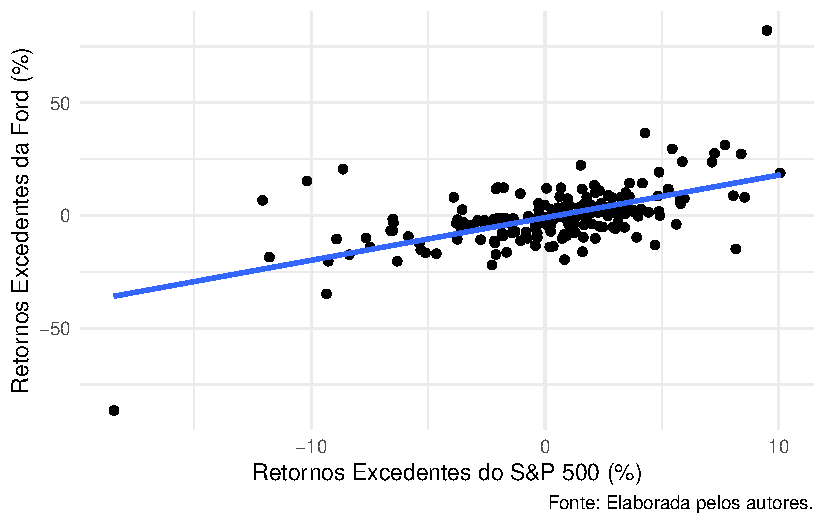
\includegraphics{01_capm_files/figure-pdf/fig-dispersao-1.pdf}

}

\caption{\label{fig-dispersao}Gráfico de Dispersão entre os retornos
excedentes da Ford e do índice S\&P (500).}

\end{figure}%

\section{Resultados e Discussão}\label{sec-resultados}

A Tab.~\ref{tbl-resultados} contém os resultados da estimação do CAPM
para os retornos excedentes da Ford usando a metodologia descrita na
Seção~\ref{sec-met}.

\begin{table}

\caption{\label{tbl-resultados}Resultados da Estimação do CAPM}

\centering{

\centering
\begin{tabular}[t]{lc}
\toprule
  & (1)\\
\midrule
(Intercept) & \num{-0.956}\\
 & {}[\num{-2.520}, \num{0.608}]\\
 & e.p. = \num{0.793}\\
 & t = \num{-1.205}\\
 & p = \num{0.230}\\
retexc\_sp500 & \num{1.890}\\
 & {}[\num{1.512}, \num{2.268}]\\
 & e.p. = \num{0.192}\\
 & t = \num{9.862}\\
 & p = \num{<0.001}\\
\midrule
Num.Obs. & \num{193}\\
R2 & \num{0.337}\\
R2 Adj. & \num{0.334}\\
F & \num{97.258}\\
\bottomrule
\multicolumn{2}{l}{\rule{0pt}{1em}Fonte: Elaborada pelos autores.}\\
\end{tabular}

}

\end{table}%

\section{Conclusões}\label{sec-conclusoes}

\section*{Referências}\label{referuxeancias}
\addcontentsline{toc}{section}{Referências}

\phantomsection\label{refs}
\begin{CSLReferences}{0}{0}
\bibitem[\citeproctext]{ref-lintner1965}
LINTNER, J. \href{https://doi.org/10.2307/1924119}{The Valuation of Risk
Assets and the Selection of Risky Investments in Stock Portfolios and
Capital Budgets}. \textbf{Review of Economics and Statistics}, v. 47, n.
1, p. 13--37, 1965.

\bibitem[\citeproctext]{ref-mossin1966capm}
MOSSIN, J. \href{https://doi.org/10.2307/1910098}{Equilibrium in a
Capital Asset Market}. \textbf{Econometrica}, v. 34, n. 4, p. 768--783,
1966.

\bibitem[\citeproctext]{ref-sharpe1964capm}
SHARPE, W. F. \href{https://doi.org/10.2307/2977928}{Capital Asset
Prices: A Theory of Market Equilibrium under Conditions of Risk}.
\textbf{Journal of Finance}, v. 19, n. 3, p. 425--442, 1964.

\bibitem[\citeproctext]{ref-treynor1961}
TREYNOR, J. L. Towards a Theory of Market Value of Risky Assets.
\textbf{Unpublished manuscript}, 1961.

\end{CSLReferences}




\end{document}
